%%%%%%%%%%%%%%%%%%%%%%%%%%%%%%%%%%%%%%%%%%%%%%%%%%%%%%%%%%%%%%%%%%%%%%%%%%%%%%%%%%%%%%%%%%%%%%%%%%%%%%%%%%%%%%%
\chapter{Some interesting results}
%%%%%%%%%%%%%%%%%%%%%%%%%%%%%%%%%%%%%%%%%%%%%%%%%%%%%%%%%%%%%%%%%%%%%%%%%%%%%%%%%%%%%%%%%%%%%%%%%%%%%%%%%%%%%%%

\section{with the wave equation}
%%%%%%%%%%%%%%%%%%%%%%%%%%%%%%%%%%%%%%%%%%%%%%%%%%%%%%%%%%%%%%%%%%%%%%%%%%%%%%%%%%%%%%%%%%%%%%%%%%%%%%%%%%%%%%%
The energy has already been considered quite thoroughly, but there are still interesting factors to consider. This chapter will discus how the different methods compare in relation to computation time, number of iterations, and error. The \texttt{wave} framework will be used due to the need for comparing the difficulty of solving the problem with different sizes.\\
!!!!!!!!!!!!!!!!!!!!!Dette må gjøres for andre problemer, dette er jo bare teit!!!!!!!!!!!!!!!!!!!!!!!\\



\begin{figure}[H]
        \centering
        \begin{subfigure}[b]{0.45\textwidth}
                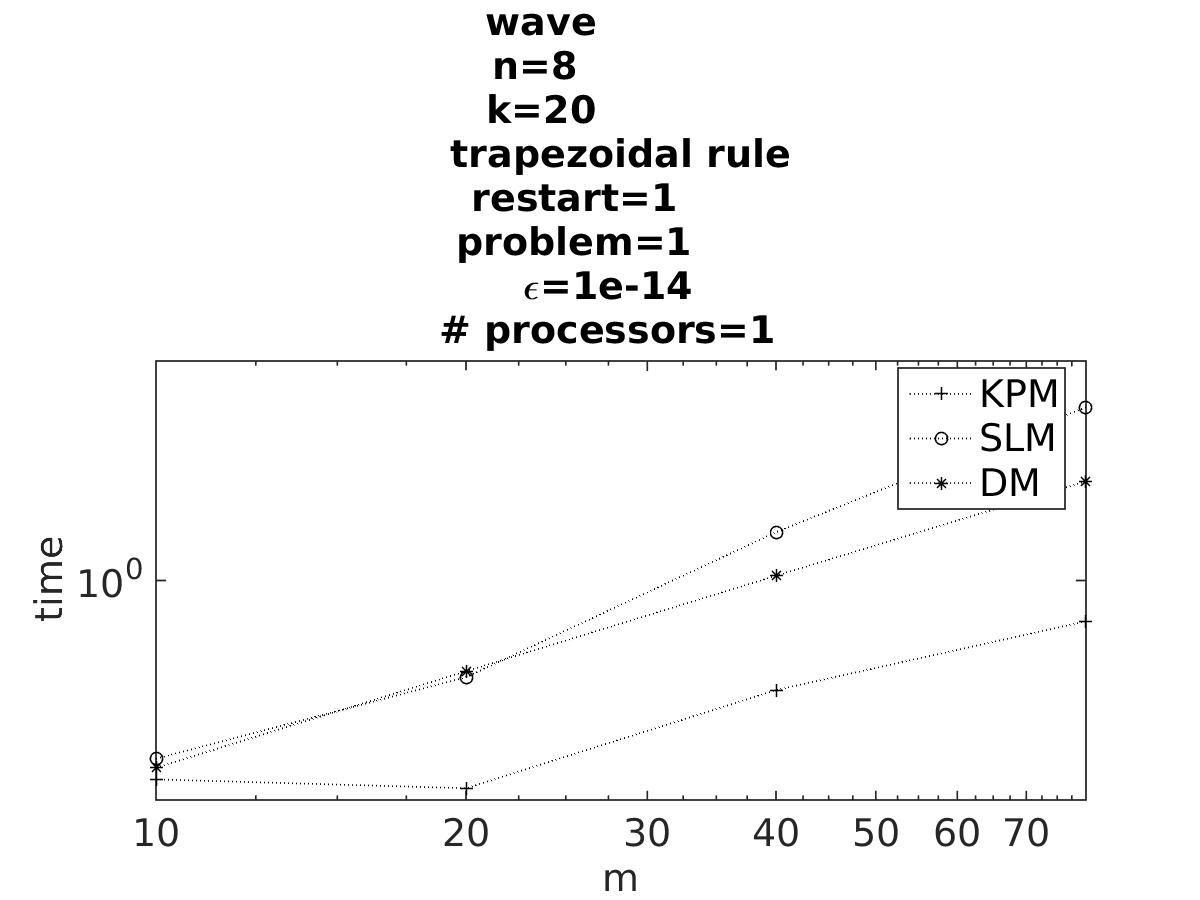
\includegraphics[width=\textwidth]{../MATLAB/fig/resulttimem.jpg}
                \caption{  }
                \label{fig:resulttimem}
        \end{subfigure}
        ~
        \begin{subfigure}[b]{0.45\textwidth}
                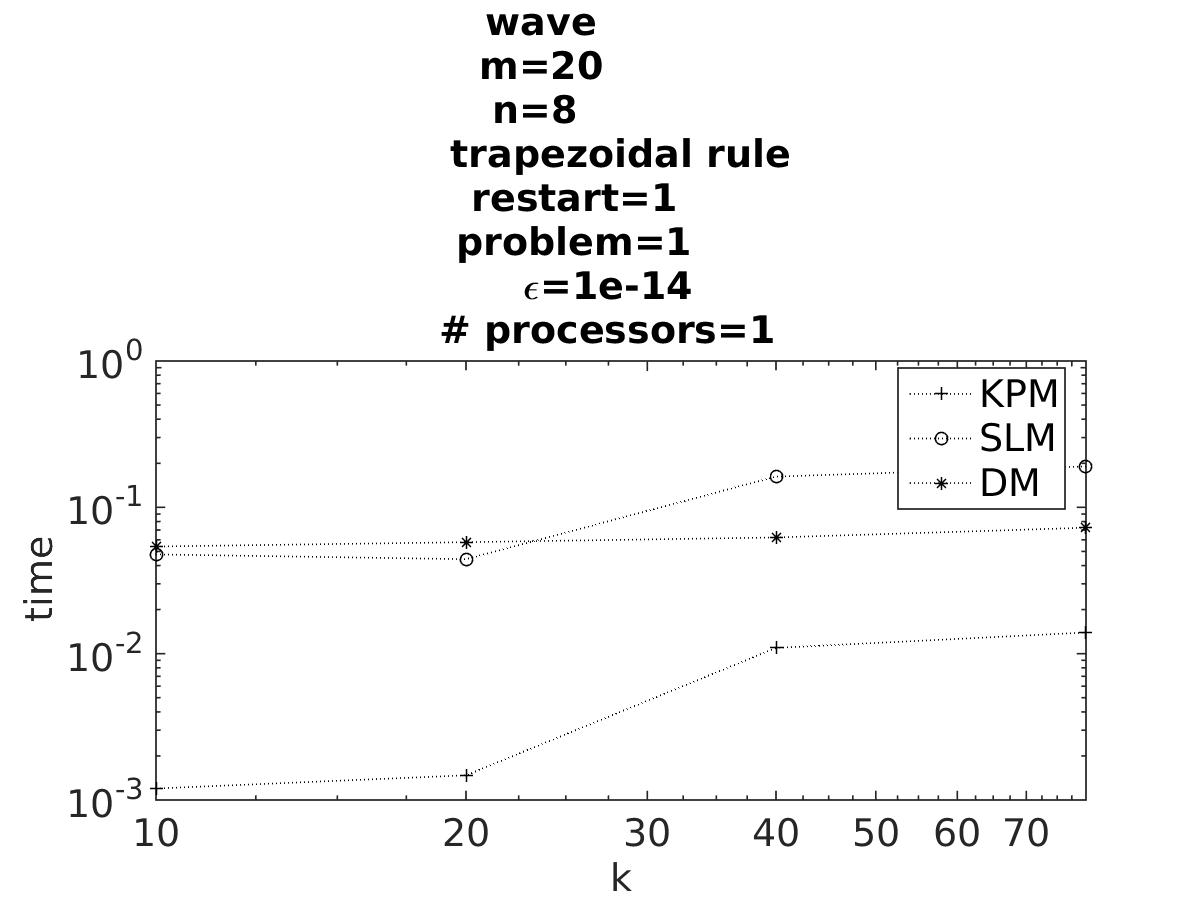
\includegraphics[width=\textwidth]{../MATLAB/fig/resulttimek.jpg}
                \caption{  }
                \label{fig:resulttimek}
        \end{subfigure}
        \caption{ For both cases KPM is faster than the other, and with DM faster than SLM.  }
        \label{fig:resulttime}
\end{figure}



\begin{figure}[H]
        \centering

                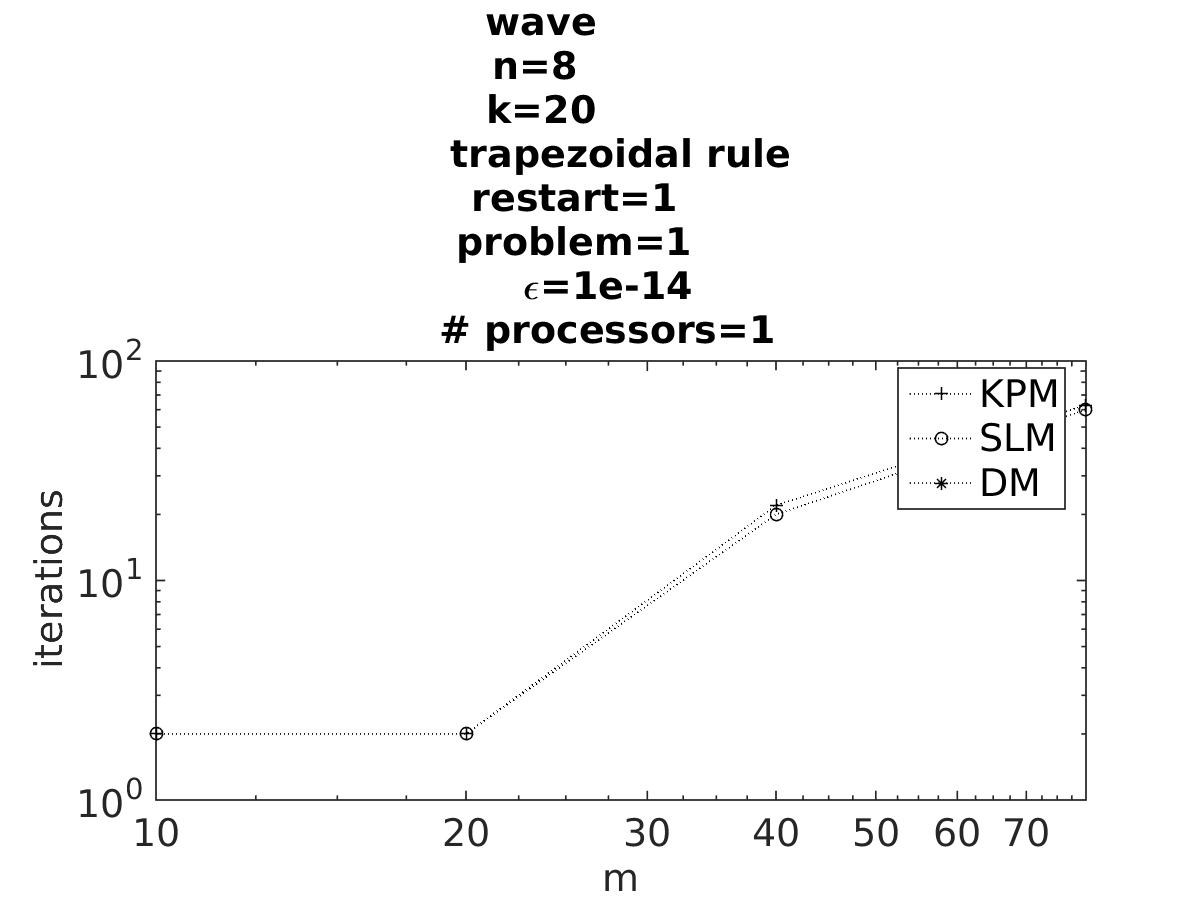
\includegraphics[width=0.45\textwidth]{../MATLAB/fig/resultiter.jpg}
        \label{fig:resultiter}
        \caption{The number of iterations are almost equal for the two methods.}
\end{figure}

\begin{figure}[H]
        \centering
        \begin{subfigure}[b]{0.45\textwidth}
                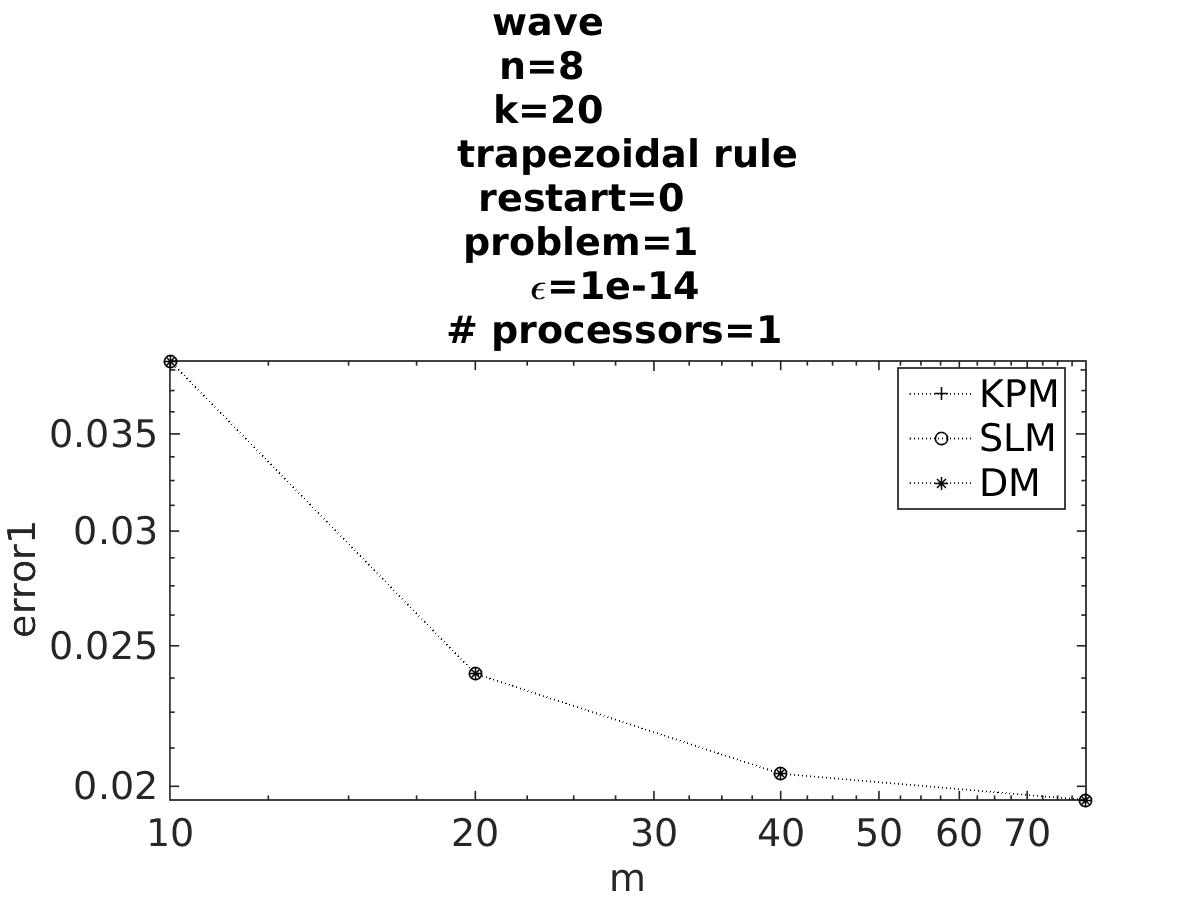
\includegraphics[width=\textwidth]{../MATLAB/fig/resulterrorr.jpg}
                \caption{  }
                \label{fig:resulterror1}
        \end{subfigure}
        ~
        \begin{subfigure}[b]{0.45\textwidth}
                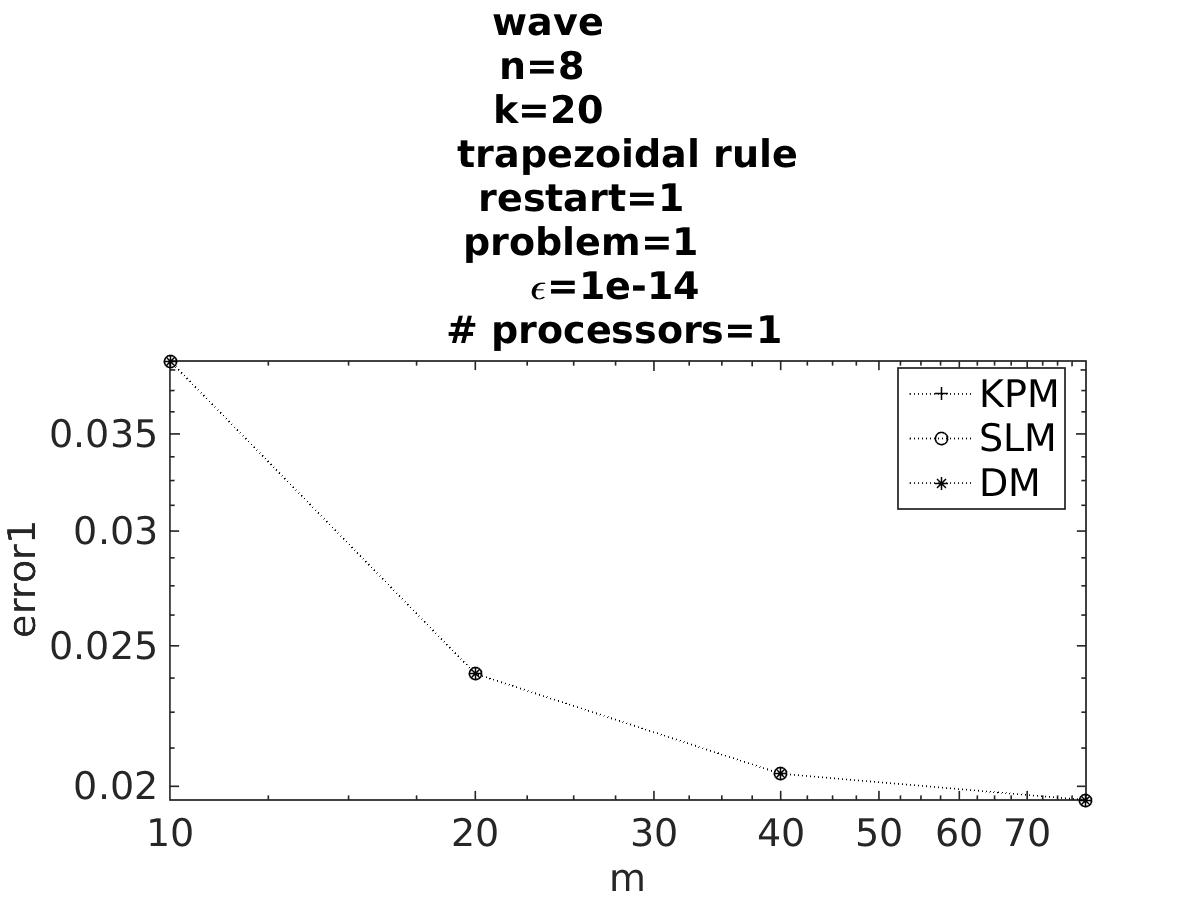
\includegraphics[width=\textwidth]{../MATLAB/fig/resulterror.jpg}
                \caption{  }
                \label{fig:resulterror2}
        \end{subfigure}
        \caption{ The error is nearly identical.  }
        \label{fig:resulterror}
\end{figure}


\begin{figure}[H]
        \centering
        \begin{subfigure}[b]{0.45\textwidth}
                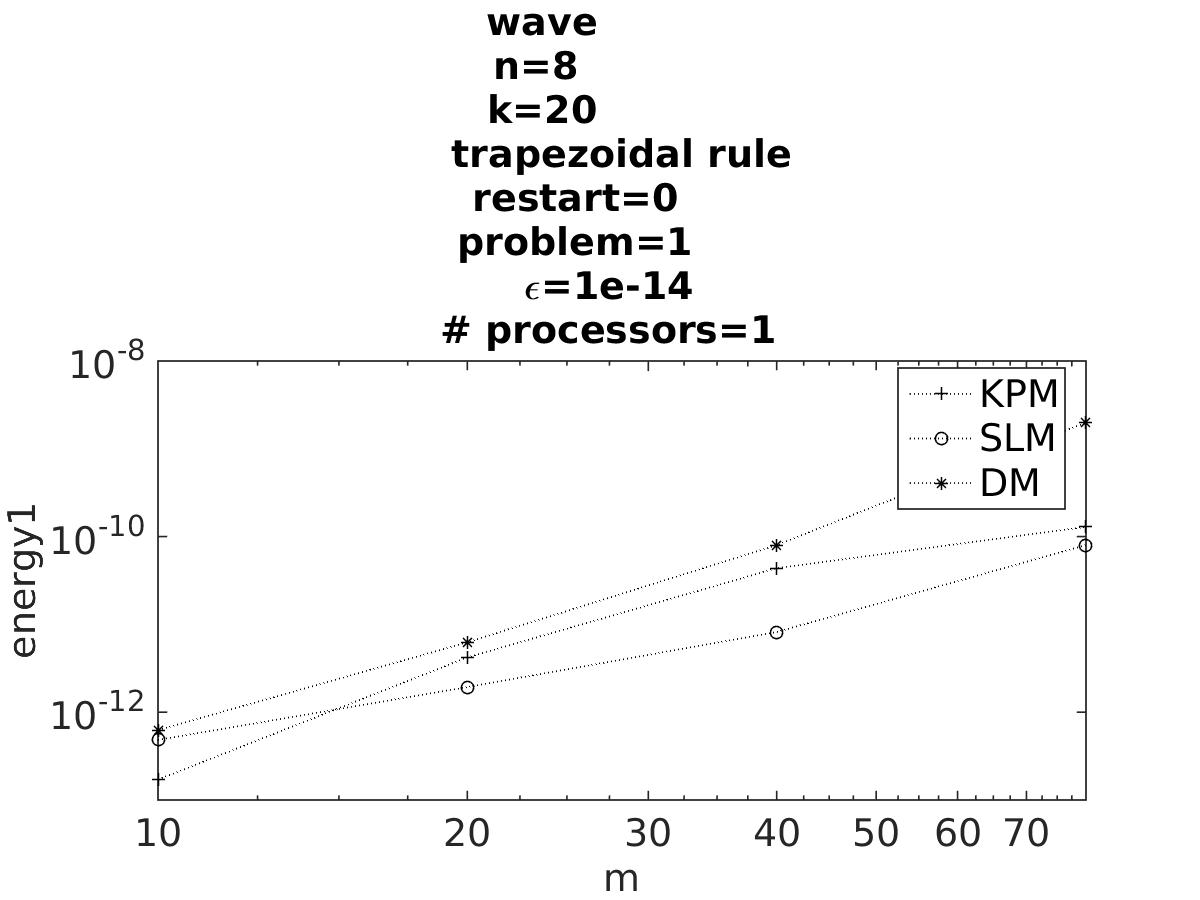
\includegraphics[width=\textwidth]{../MATLAB/fig/resultenergyr.jpg}
                \caption{  }
                \label{fig:resultenergy1}
        \end{subfigure}
        ~
        \begin{subfigure}[b]{0.45\textwidth}
                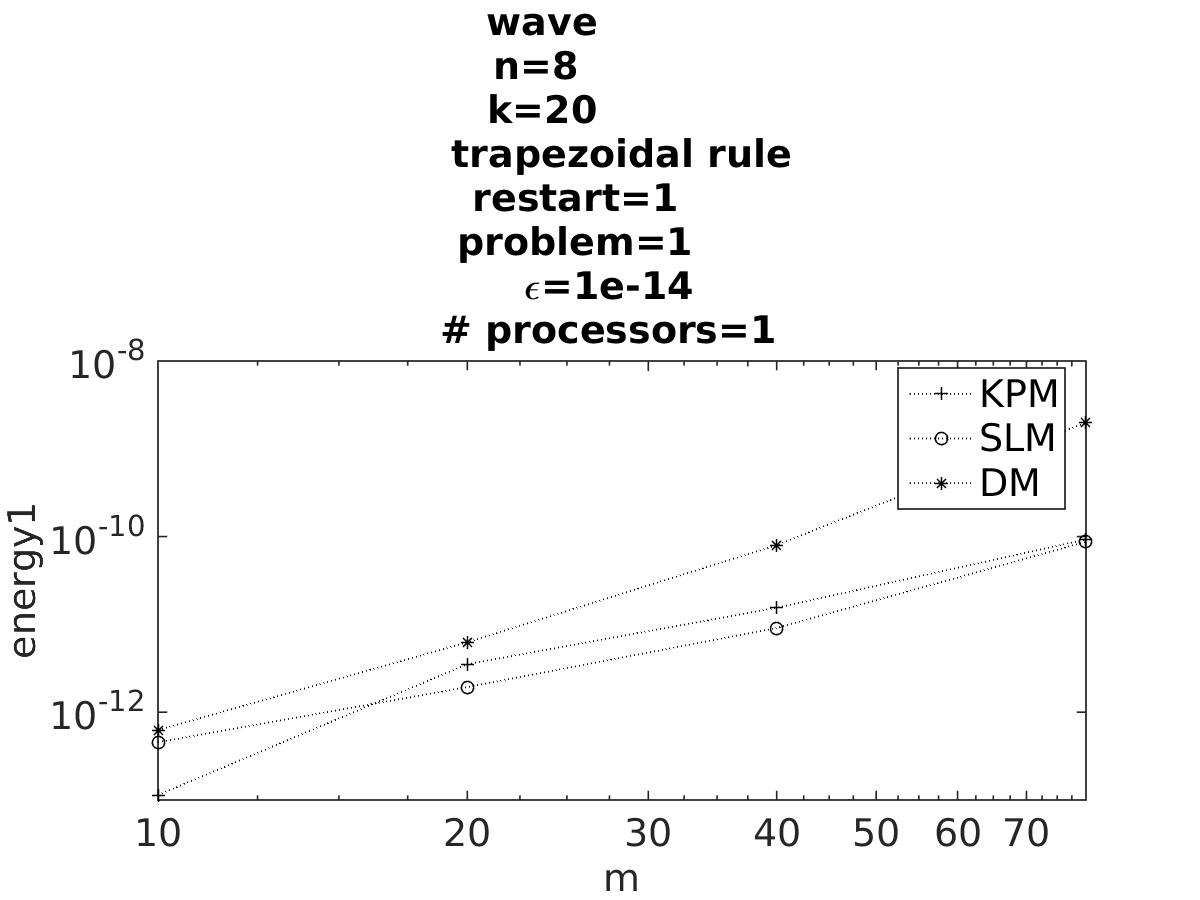
\includegraphics[width=\textwidth]{../MATLAB/fig/resultenergy.jpg}
                \caption{  }
                \label{fig:resultenergy2}
        \end{subfigure}
        \caption{ SLM and KPM has the best energy estimation, with DM not far behind. }
        \label{fig:resultenergy}
\end{figure}





\section{with the semirandom equation}
%%%%%%%%%%%%%%%%%%%%%%%%%%%%%%%%%%%%%%%%%%%%%%%%%%%%%%%%%%%%%%%%%%%%%%%%%%%%%%%%%%%%%%%%%%%%%%%%%%%%%%%



\begin{figure}[H]
        \centering
        \begin{subfigure}[b]{0.45\textwidth}
                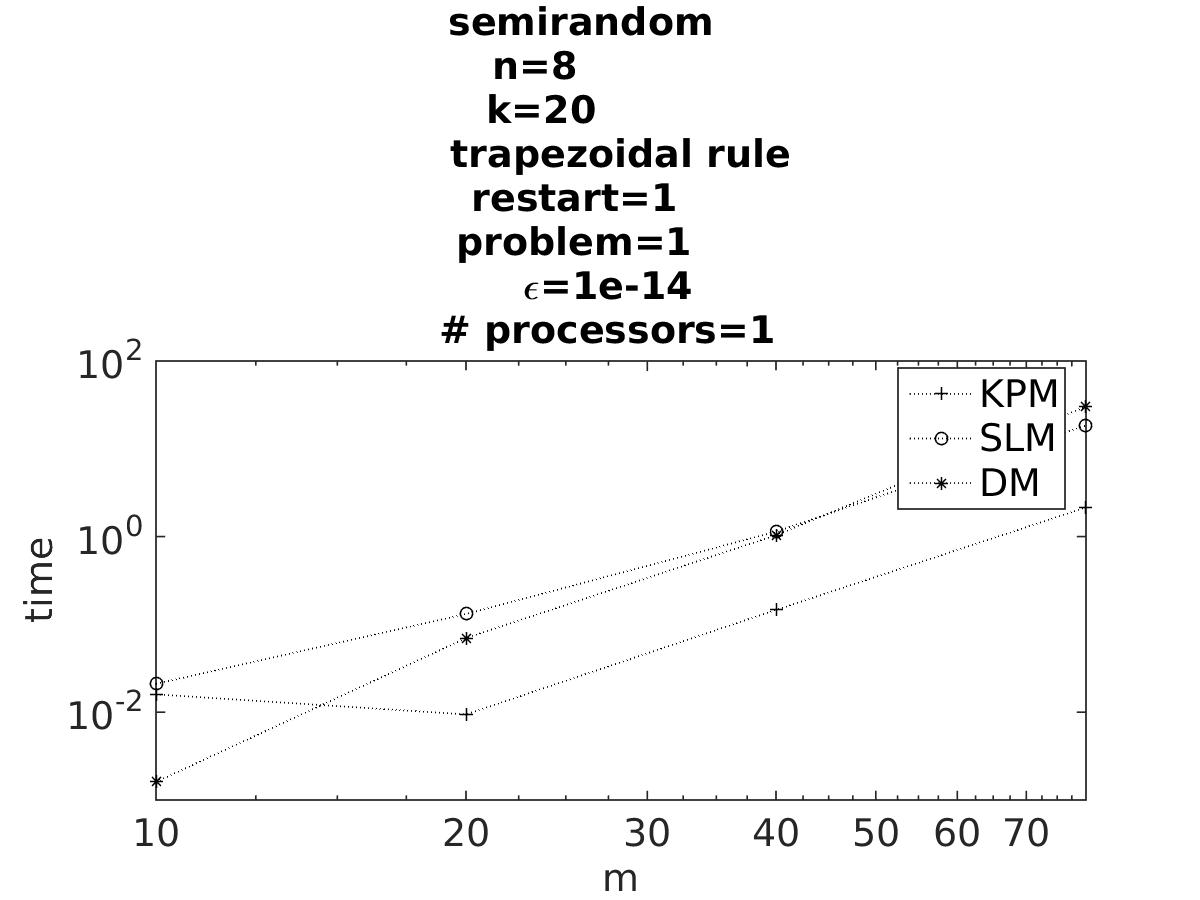
\includegraphics[width=\textwidth]{../MATLAB/fig/sresulttimem.jpg}
                \caption{  }
                \label{fig:sresulttimem}
        \end{subfigure}
        ~
        \begin{subfigure}[b]{0.45\textwidth}
                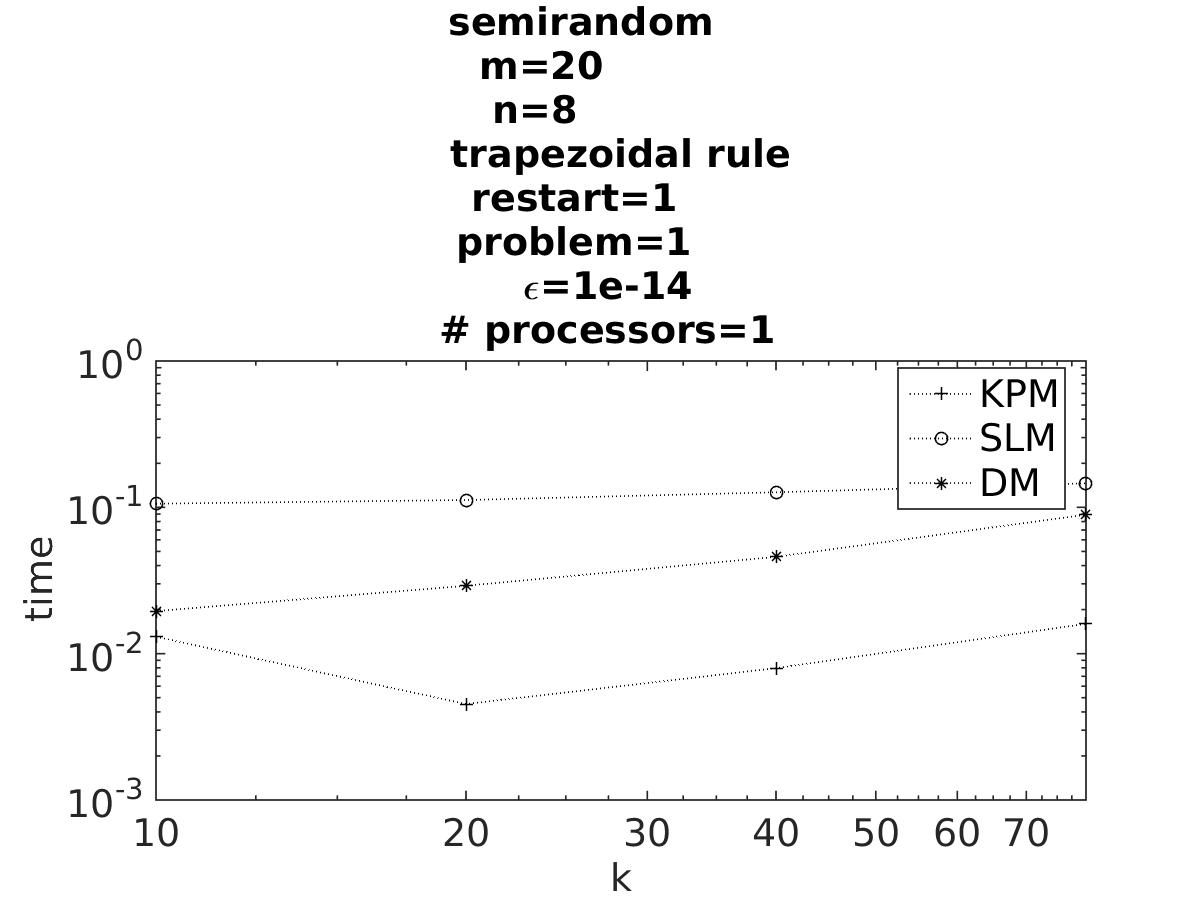
\includegraphics[width=\textwidth]{../MATLAB/fig/sresulttimek.jpg}
                \caption{  }
                \label{fig:sresulttimek}
        \end{subfigure}
        \caption{ For both cases KPM is faster than the other, and with DM faster than SLM.  }
        \label{fig:sresulttime}
\end{figure}



\begin{figure}[H]
        \centering

                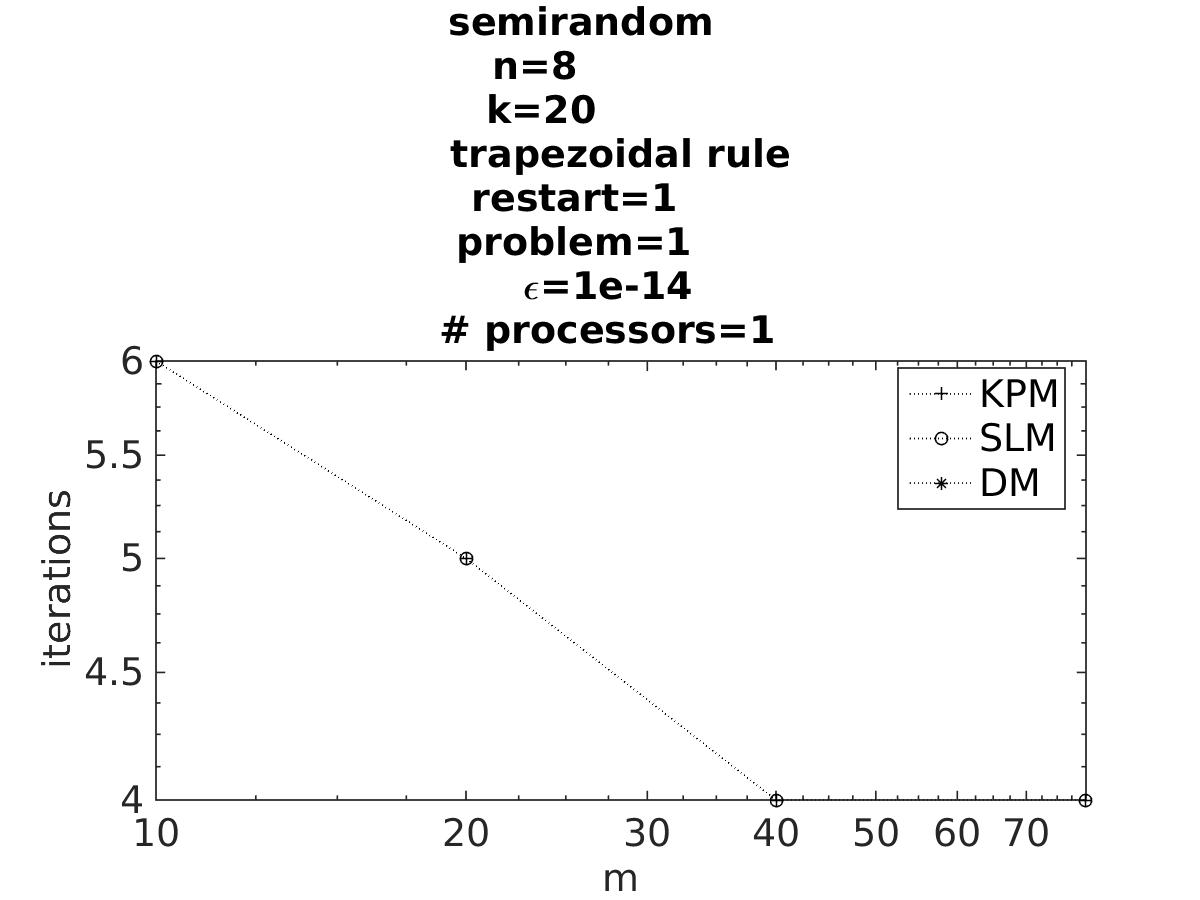
\includegraphics[width=0.45\textwidth]{../MATLAB/fig/sresultiter.jpg}
        \label{fig:sresultiter}
        \caption{The number of iterations are almost equal for the two methods.}
\end{figure}

\begin{figure}[H]
        \centering
        \begin{subfigure}[b]{0.45\textwidth}
                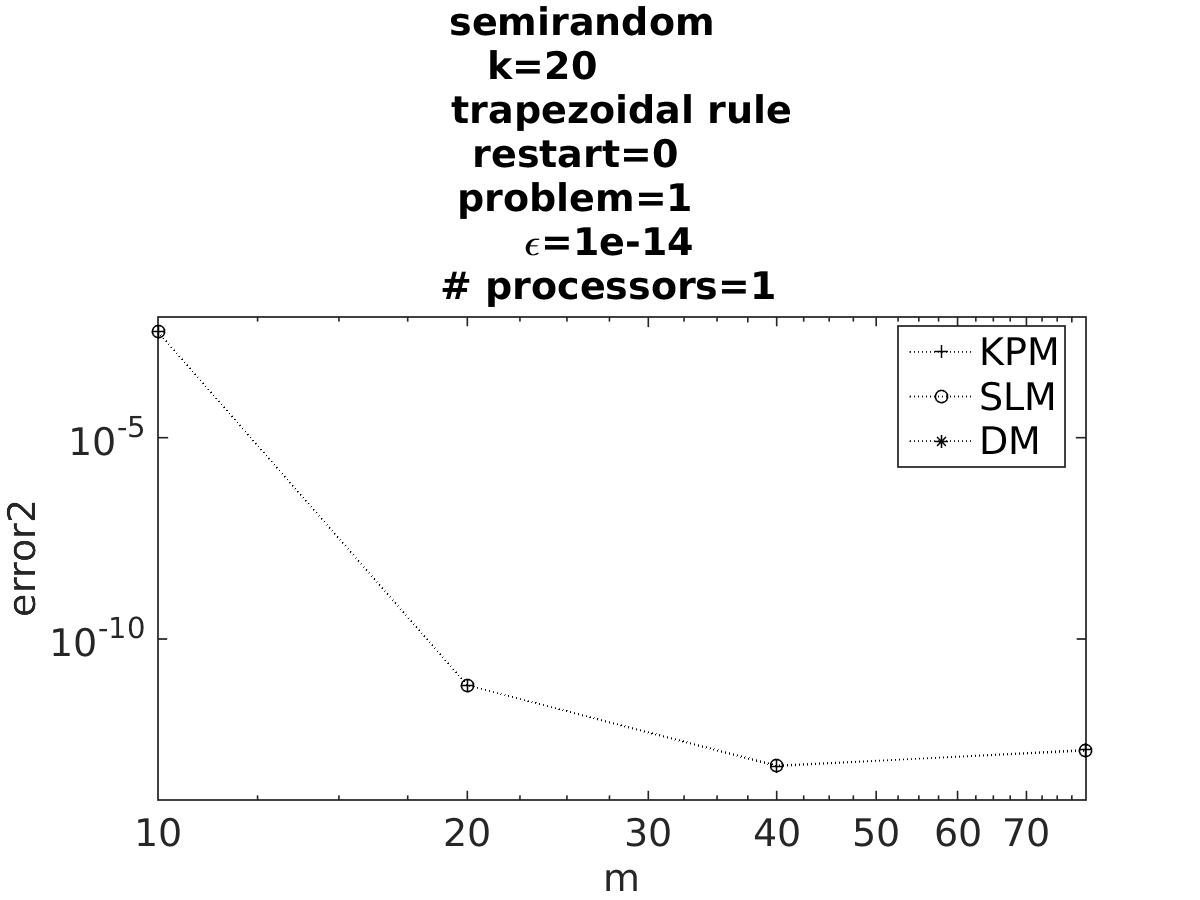
\includegraphics[width=\textwidth]{../MATLAB/fig/sresulterrorr.jpg}
                \caption{  }
                \label{fig:sresulterror1}
        \end{subfigure}
        ~
        \begin{subfigure}[b]{0.45\textwidth}
                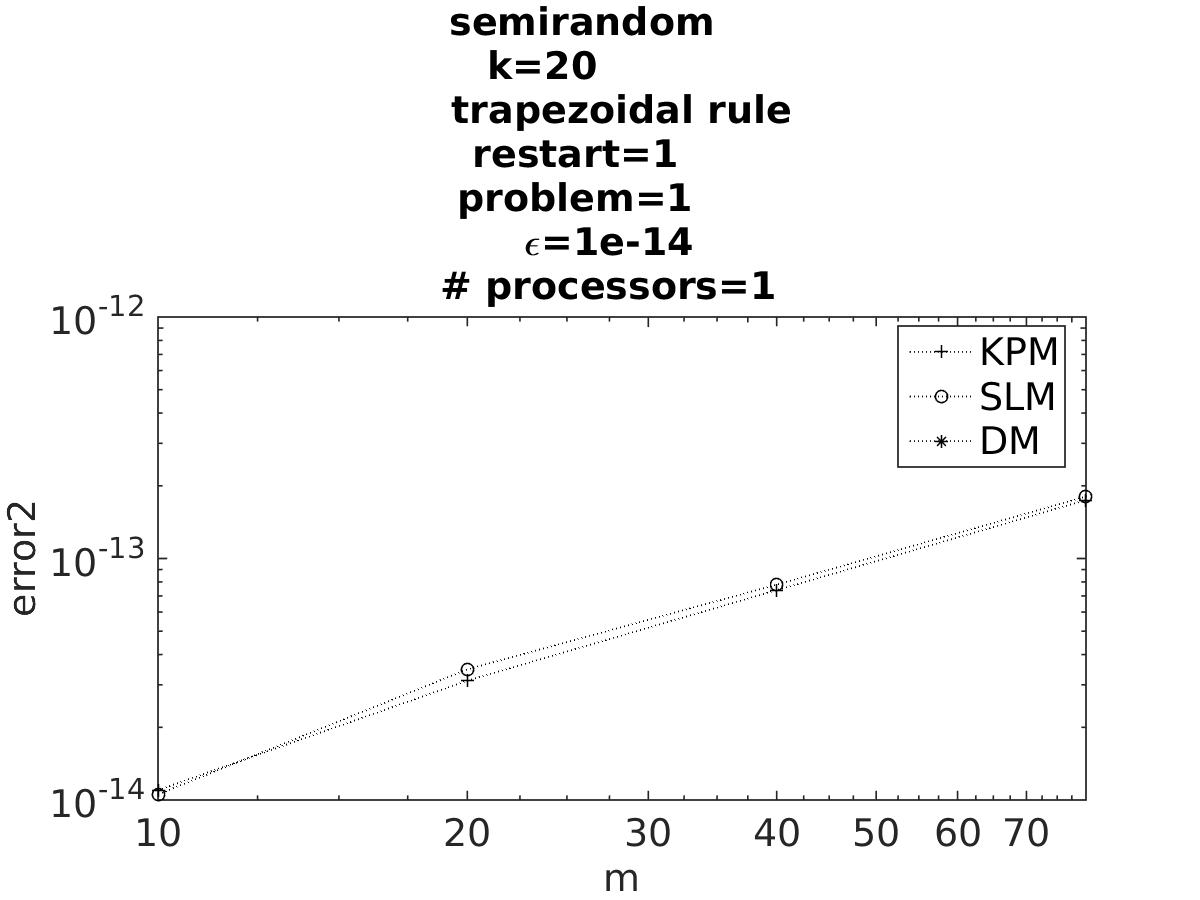
\includegraphics[width=\textwidth]{../MATLAB/fig/sresulterror.jpg}
                \caption{  }
                \label{fig:sresulterror2}
        \end{subfigure}
        \caption{ The error is nearly identical.  }
        \label{fig:sresulterror}
\end{figure}


\begin{figure}[H]
        \centering
        \begin{subfigure}[b]{0.45\textwidth}
                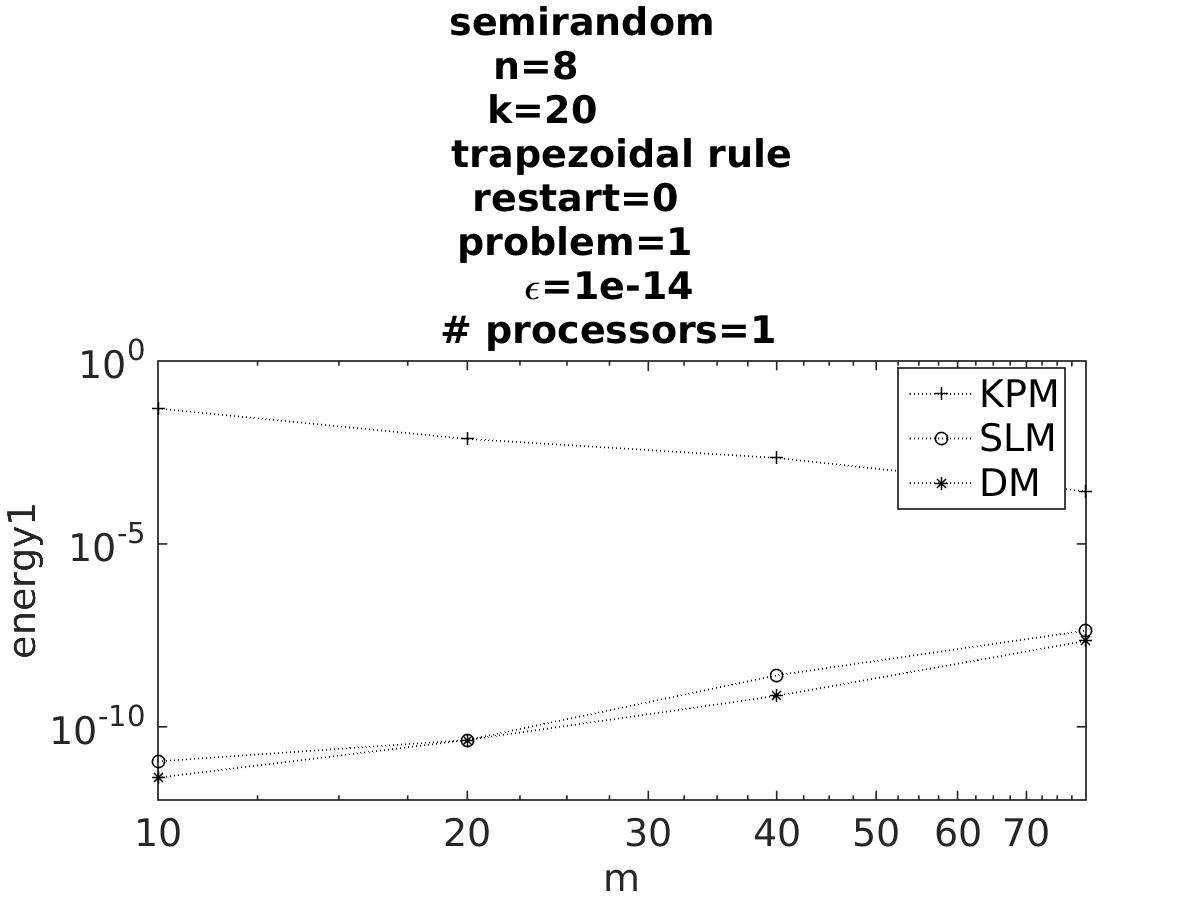
\includegraphics[width=\textwidth]{../MATLAB/fig/sresultenergyr.jpg}
                \caption{  }
                \label{fig:sresultenergy1}
        \end{subfigure}
        ~
        \begin{subfigure}[b]{0.45\textwidth}
                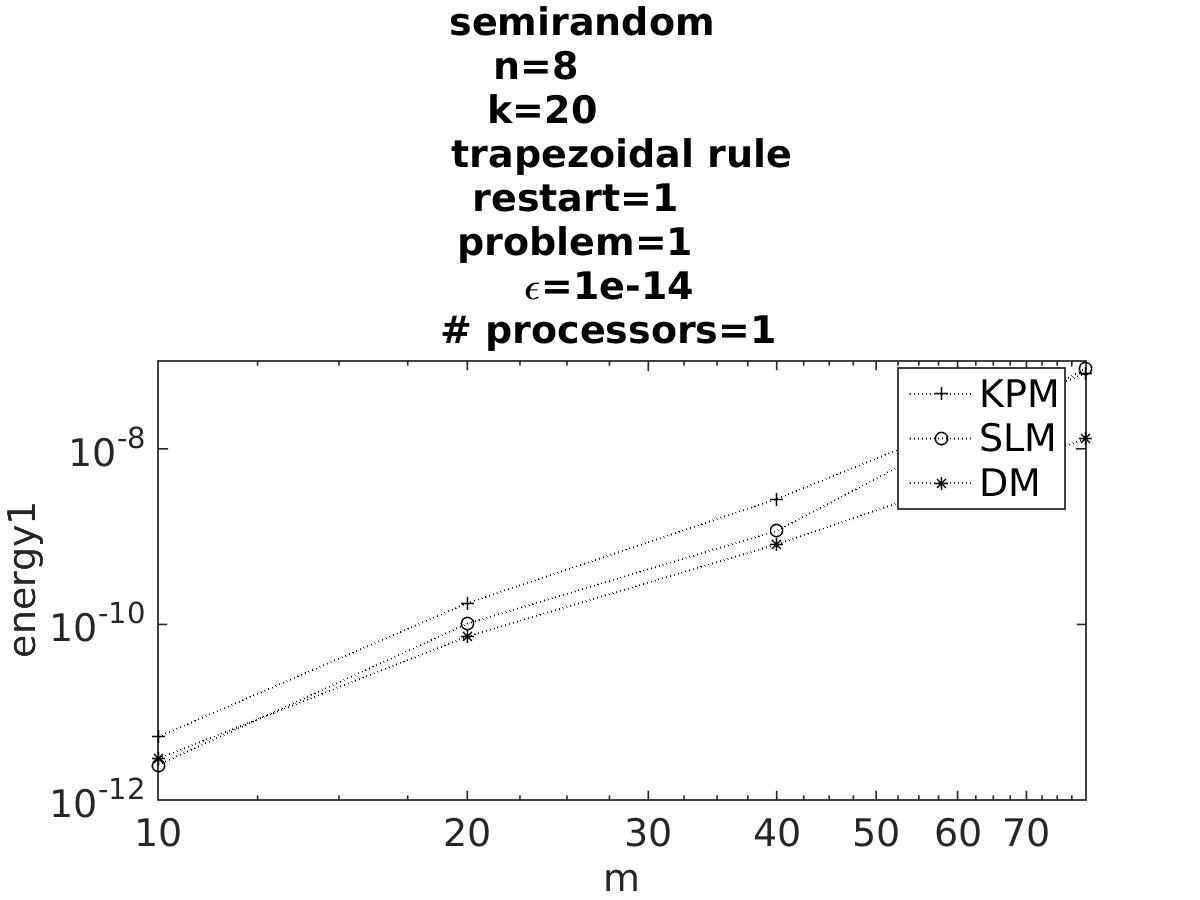
\includegraphics[width=\textwidth]{../MATLAB/fig/sresultenergy.jpg}
                \caption{  }
                \label{fig:sresultenergy2}
        \end{subfigure}
        \caption{ SLM and KPM has the best energy estimation, with DM not far behind. }
        \label{fig:sresultenergy}
\end{figure}

